\chapter{Introducción}

    \section{Motivación}
    \label{intro:motiv}

        Actualmente, los juegos de mesa han pasado a un segundo -o incluso tercer- plano frente a otras formas de entretenimiento más modernas y dinámicas: los videojuegos, cada vez más realistas e inmersivos, y los servicios de series y películas, cuyo contenido se amplía tras cada estreno o exclusiva, son los principales alicientes para que los juegos de mesa, poco a poco, se vuelvan un tema menos frecuente del que hablar.

        % TODO: expandir un poco más.

        Sin embargo, siguen existiendo personas cuya principal afición es juntarse alrededor de un buen juego, comunicarse y mantener ese contacto e interacción que ofrece una partida en vivo.

        Tras comentar esta situación, sucede que en bastantes ocasiones, precisamente por esa escasez de jugadores activos:

        \begin{itemize}

            \item Si se establece un juego de mesa determinado, no siempre se alcanza el número mínimo o adecuado de jugadores.
            \item Si hay jugadores más que suficientes, suele ser difícil elegir el juego de mesa debido a la gran cantidad de opciones.

        \end{itemize}

        Para resolver esos dos inconvenientes, se plantea crear una herramienta en formato de aplicación Android que facilite el descubrimiento (y posterior conexión) de personas con las que organizar partidas de juegos de mesa, para que puedan reunirse y jugar, y cuya principal función sea la de descubrir partidas cercanas mediante geolocalización.

        \newpage


    \section{Objetivos}

        % TODO: revisar toda la sección.

        Como se comentó en la sección anterior \ref{intro:motiv}, este trabajo de fin de grado pretende reducir o resolver los inconvenientes previamente planteados creando una aplicación Android simple que permita a sus usuarios:

        \begin{itemize}

            \item Registrarse y establecer sus preferencias geográficas para descubrir partidas.
            \item Añadir y eliminar a otros usuarios a su lista de amigos.
            \item Añadir y eliminar juegos de mesa asociados a sus cuentas.
            \item Crear y eliminar partidas que usan los juegos de mesa asociados a las cuentas.
            \item Unirse a partidas organizadas por amigos u otros usuarios que hayan sido descubiertas por las preferencias geográficas.

        \end{itemize}

        \vskip 1 cm

        La aplicación hará uso de una base de datos que gestionará la información de los usuarios, los juegos registrados y las partidas creadas. Por tanto, también se realizará una base de datos capaz de:

        \begin{itemize}

            \item Registrar diferentes juegos de mesa y gestionar las nuevas entradas.
            \item Registrar diferentes partidas y sus participantes (jugadores).
            \item Registrar diferentes usuarios y sus contraseñas.

        \end{itemize}

        \vskip 1 cm

        La conexión entre la aplicación y la base de datos es lo produce el efecto final esperado.

        \newpage


    \section{Estado del arte}

        En relación a los juegos de mesa, la idea de descubrir y conectar con otras personas no es nueva: durante el desarrollo de Internet han ido surgiendo herramientas que cumplen este fin, ya sea de forma central o como una de las muchas posibilidades que ofrece un servicio; pero no siempre ha sido así y de hecho, como se mencionó en la sección de Motivación \ref{intro:motiv}, la clave de los juegos de mesa es el contacto y la cercanía real, por lo que tiene sentido que antes de toda esta digitalización la gente conociera a otras personas con las que jugar.

        Es decir, los jugadores no están totalmente aislados en absoluto, la posibilidad siempre ha estado ahí.


        \subsection{Medios tradicionales}

            El fin común de estos medios es reunir gente físicamente entorno a un acontecimiento o evento, lo que permite a las personas interaccionar entre ellas y conocer nuevos jugadores potenciales y nuevos juegos de mesa.

            \paragraph{Tiendas de juegos de mesa}

                Es común en muchas tiendas programar eventos de cierto juego en concreto o incluso dedicar un día a la semana para organizar encuentros libres, donde las personas asisten solas o con amigos para jugar allí en un ambiente mucho más inmersivo y con la posibilidad de conocer a gente nueva interesada en el hobby que también esté participando al mismo tiempo.

            \paragraph{Convenciones}

                % TODO: revisar más tarde.

                Estos eventos que tienen lugar normalmente una vez al año, reúnen a muchísimas personas de la zona donde se realizan y sus alrededores. Además, debido al tamaño del evento, suelen atraer a gente que no está especialmente ligada al hobby, por lo que fomenta su descubrimiento.

                Las personas que acuden a las convenciones se encuentran con zonas de juegos habilitadas para probar los últimos títulos, conocer grupos interesados y participar en torneos que tiene lugar durante la duración de la convención.


        \subsection{Medios digitales}

            El fin común de estos medios es descubrir y conectar a personas interesadas en los juegos de mesa, para que puedan reunirse físicamente y jugar partidas; a diferencia de los medios tradicionales, se centran más en la inmediatez.

            % TODO: expandir ampliamente todos los medios posibles y modificar la bibliografía.

            \paragraph{BoardGameGeek}

                Esta página web \cite{BGG} creada en el año 2000 contiene una enorme base de datos de juegos de mesa y permite a sus usuarios registrarse, dando lugar a funciones básicas de redes sociales como el intercambio de mensajes y la creación de eventos que, en este caso, tienen lugar en forma de partidas o sesiones de juegos de mesa.

                Podría considerarse por todos aquellos jugadores habituales como la biblioteca de Alejandría \cite{Biblioteca-Alejandria} de los juegos de mesa: si un juego existe, por extraño, limitado y raro que sea, es posible que alguien ya lo haya añadido a la base de datos.

                \subparagraph{Funciones}

                    Crear usuarios, registrar juegos de mesa en la plataforma, asociar juegos de mesa a los usuarios, definir encuentros entre usuarios, intercambio de mensajes entre usuarios...

            \paragraph{Discord}

                Actualmente una de las aplicaciones más populares (si no la más popular) de comunicación VOIP e intercambio de mensajes \cite{Discord}. Iniciando en 2015 con el fin de sobrepasar a Skype y TeamSpeak en el territorio de la comunicación en videojuegos, sufrió un gran incremento de uso diario dirante los años de la pandemia del COVID-19, lo que hizo que aumentaran sus capacidades y funcionalidades, por lo que terminó convirtiéndose en una aplicación de comunicación multipropósito.

                Precisamente esa familiaridad con el programa, su amplio número de usuarios y su alta flexibilidad, han permitido que sea posible gestionar partidas de juegos de mesa y otras comunidades que giren alrededor de este hobby.

                Cabe destacar que esta aplicación es mayormente usada por gente joven y aquellos relacionados con la informática.

                \subparagraph{Funciones}

                    Crear usuarios, crear o unirse a servidores, crear o unirse a canales de texto o de voz, gestión de permisos con roles, intercambio de mensajes con formato Markdown entre usuarios, comunicación por voz y/o vídeo entre usuarios...


            \paragraph{Facebook}

                Una de las redes sociales más famosa del mundo, con miles de millones de usuarios.

                Esta plataforma permite la creación de grupos y eventos, por lo que existen diversos grupos locales de juegos de mesa donde la gente puede participar y quedar para jugar.

                \subparagraph{Funciones}

                    Crear usuarios, crear publicaciones, crear o unirse a grupos, crear o unirse a eventos, intercambio de mensajes entre usuarios...

                    \newpage


    \section{Metodología del trabajo empleada}
    \label{intro:met}

        Para la elaboración de este proyecto se ha empleado un \textbf{desarrollo incremental}, que consiste en, partiendo de una base, añadirle sucesivas mejoras sin que estas perjudiquen al resto del proyecto desarrollado hasta el momento.

        % TODO: revisar más tarde cómo está expresado esto.

        Al tratarse del desarrollo de un software, era imprescindible -y prácticamente, trivial- el uso de un controlador de versiones, para el que se ha elegido trabajar con Git y Github; y además, se ha hecho uso de la funcionalidad de \textit{Proyectos} que ofrece esta plataforma.

        % TODO: ¿Mencionar también Git y Github?

        \subsection{Tableros Kanban}

            Este método consiste en la clasificación de tareas (tarjetas) en diferentes estados (columnas) a medida que se trabaja en cada una de ellas. Su simpleza y su flexibilidad permite que pueda aplicarse a flujos de trabajos ya implementados como medida adicional de progreso y organización.

            Como se mencionó en la sección \ref{intro:met}, Github ofrece una función de visualización de proyectos, que resultan ser como tableros Kanban, que pueden ser manuales (como en este caso) o automatizados con los \textit{Issues} de esa misma plataforma.

            \begin{figure*}[h]

                \centering
                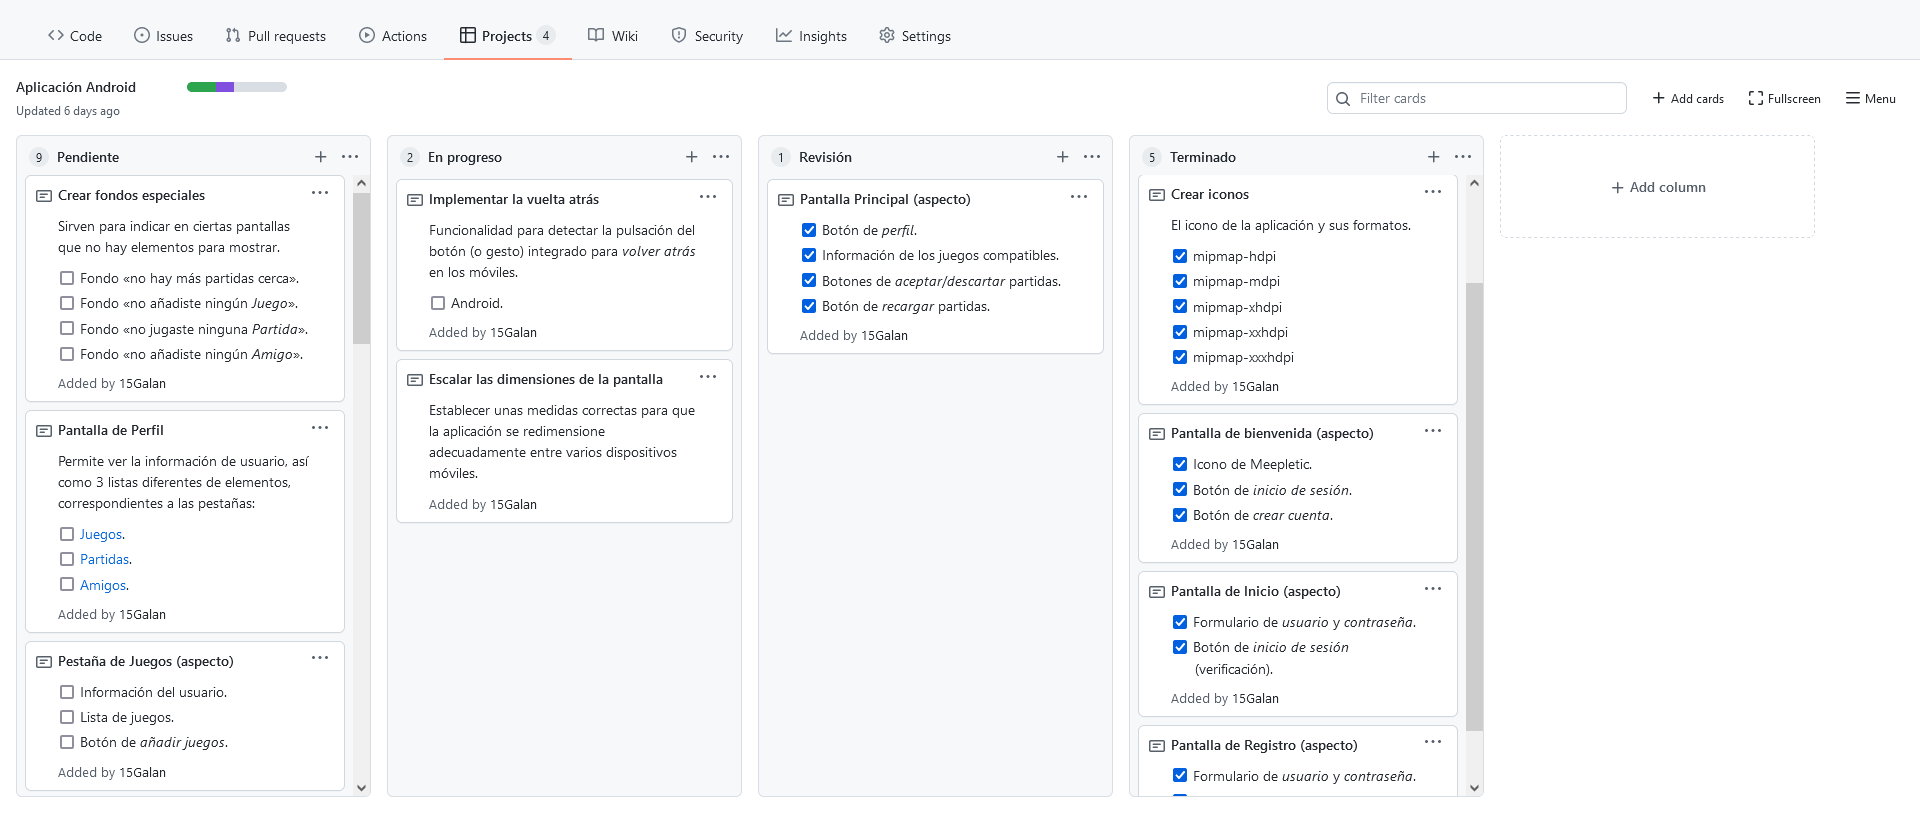
\includegraphics[scale=0.2]{images/progreso-app.png}
                \caption{\textit{Proyecto} de Github de la aplicación Android}

            \end{figure*}

            La composición elegida para todos los tableros Kanban del proyecto ha sido:

            \begin{itemize}

                \item \textbf{Pendientes}: tareas que aún no han sido tratadas de ninguna forma. Corresponden a conceptos nacidos de lluvias de ideas o que representan requisitos de la aplicación.

                \item \textbf{En Progreso}: tareas que están siendo trabajadas. No debe trabajarse en demasiadas tareas a la vez o puede producirse un cuello de botella en el desarrollo.

                \item \textbf{Revisión}: tareas que han sido completadas, pero que requieren un último vistazo para probar que verdaderamente están listas y no necesitan más atención.

                \item \textbf{Completadas}: tareas que han sido trabajadas y revisadas. Terminadas definitivamente.

            \end{itemize}

            \newpage


            Esta herramienta también incluye una pequeña barra de progreso -que debe activarse en el menú del \textit{Proyecto}- y permite al usuario verificar el estado de las tareas, según el tablero descrito: en verde, las tareas marcadas como terminadas; en morado, las tareas en progreso o que necesitan revisión. Este diseño bicolor favorece la interpretación de una forma simple y directa.

            \begin{figure*}[h]
            \label{figura:proyectos}

                % TODO: revisar el comentario de la figura.

                \centering
                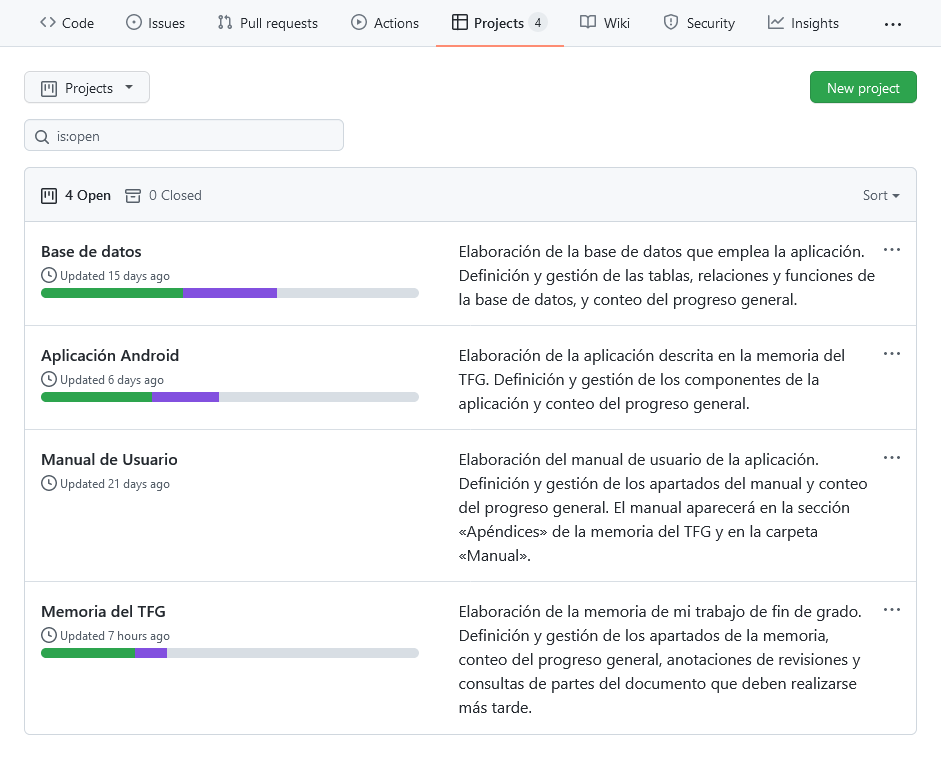
\includegraphics[scale=0.35]{images/progreso-resumen.png}
                \caption{Resumen del desarrollo del proyecto, dividido en \textit{Proyectos}}

            \end{figure*}

            \newpage


    % TODO: ¿Hasta qué punto es necesario explicar la estructura habiendo un índice?

    \section{Estructura de la memoria}

        Este documento está dividido en capítulos correspondientes a las fases de desarrollo que se establecieron para llevar a cabo el proyecto, exceptuando aquellos que dan forma propia de memoria de trabajo de fin de grado, como son la introducción y las conclusiones finales:

        \begin{itemize}

            \item \textbf{Capítulo de introducción}: el capítulo actual, contiene el preámbulo formal donde se describe la idea y el contenido de este documento.

            \item \textbf{Capítulo de investigación y estudio}: describe la fase previa a la implementación de la aplicación donde se analizaron distintas herramientas con el objetivo de aplicarlas al proyecto.

            \item \textbf{Capítulo de diseño}: contiene imágenes acerca del aspecto de la aplicación y diagramas sobre del funcionamiento de la misma, así como una descripción de los requisitos.

            % TODO: revisar los "requisitos"

            \item \textbf{Capítulo de implementación}: describe el proceso de creación de la aplicación y el establecimiento de la base de datos.

            \item \textbf{Capítulo de correcciones y mejoras}: describe la última parte del proyecto en el que la aplicación, siendo funcional, es usada y probada con el fin de mejorarse añadiendo nuevas funciones o corrigiendo fallos.

            \item \textbf{Capítulo de conclusiones}: trata acerca de los resultados obtenidos durante o tras la realización del proyecto, así como las posibles líneas futuras del mismo.

        \end{itemize}

        Finalmente, el documento cierra con la \textbf{bibliografía} y un \textbf{apéndice}, correspondiente al manual de usuario de la aplicación.


\cleardoublepage



\chapter{Investigación y estudio}

    Durante esta fase, se realizó una búsqueda de tecnologías y recursos que pudieran tener cabida en el proyecto de la aplicación Android.

    Se decidió realizar la aplicación usando el lenguaje Lua, más alejado del estándar de Android y sus frameworks que trabajan con Java o Kotlin. Junto a esa decisión, se llegó a la conclusión de usar la plataforma Solar2D, un motor de juegos para dispositivos móviles que trabaja, justamente, usando el lenguaje Lua; esta plataforma ofrece una amplia gama de librerías integradas con las que poder desarrollar juegos y proyectos, además de ser muy intuitiva, sencilla e informativa para desarrolladores con poca o ninguna experiencia en Lua, como ha sido este caso.


    \section{Aplicación Android}

        \subsection{Lua}
        \label{inv:lua}

            \nocite{Manual-Lua}

            \begin{figure*}[h]
            \label{figura:lua}

                \centering
                
\includegraphics[scale=0.05]{images/investigacion/Lua.png}
                \caption{Logo de Lua}

            \end{figure*}

            Lenguaje de programación extensible, que ofrece buen soporte tanto para programación orientada a objetos, como para la programación funcional y la programación orientada a datos. Se emplea como un lenguaje de script ligero pero potente, para que extienda cualquier programa que lo considere necesario: por tanto, al ser un lenguaje que extiende la función de otro, carece del concepto de programa principal, por lo que funciona embebido al programa anfitrión que lo utiliza.

            Según sus propios creadores, los factores que definen a Lua es su \textbf{potencia}, \textbf{eficiencia}, \textbf{ligereza} e \textbf{integración}.

            \newpage


        \subsection{Solar2D}

            \begin{figure*}[h]
            \label{figura:solar2d}

                \centering
                
\includegraphics[scale=0.6]{images/investigacion/Solar2D.png}
                \caption{Logo de Solar2D}

            \end{figure*}

            Anteriormente conocido como Corona SDK \cite{Corona-Labs}, este motor de juegos 2D usa el lenguaje Lua descrito en la sección \ref{inv:lua}, por lo que era la plataforma ideal para el desarrollo de la aplicación. Su página web amigable, su foro y su abundante documentación, convierten a Solar2D en un motor de juegos bien valorado por los desarrolladores de ese campo, ya que no solo permite que los más experimentados hagan un buen uso de su potencia, sino que aquellos usuarios más novatos puedan integrarse poco a poco y con mucha ayuda disponible en el complejo mundo de la creación de juegos para dispositivos móviles.

            Otro punto fuerte de este motor es su simulador, que permite emular el comportamiento de la aplicación que se esté desarrollando adoptando los cambios en el código casi al instante; además del simulador, ofrece una función llamada \textit{Corona Live Server} que permite trasladar dicho simulador directamente al dispositivo móvil usando la red local a la que esté conectada, esto permite ejecutar y comprobar algunas funciones no disponibles en el simulador (por ejemplo y relacionado con este proyecto, las vista de mapas de Google Maps).

            % Los módulos de Lua son como las librerías de cualquier lenguaje de programación.

            % \paragraph{Módulo}


        \subsection{IntelliJ IDEA}

            \nocite{Jetbrains-IntelliJ}

            \begin{figure*}[h]
            \label{figura:intellij}

                \centering
                
\includegraphics[scale=0.04]{images/investigacion/IntelliJ.png}
                \caption{Logo de IntelliJ IDEA}

            \end{figure*}

            Entorno de desarrollo integrado (IDE) creado por Jetbrains considerado como uno de los más usados actualmente junto a Visual Studio Code, que cuenta con una amplia cantidad de características y funcionalidades, además de compatibilidad con herramientas de desarrollo como Maven, Gradle, STS... que funcionan de forma inmediata. IntelliJ IDEA está diseñado para mejorar la productividad de sus usuarios con asistencia intuitiva para todos los lenguajes de programación y frameworks.


        \subsection{API de Google Maps}

            % TODO: completar más adelante.

            \begin{figure*}[h]
            \label{figura:api}

                \centering
                
\includegraphics[scale=0.25]{images/investigacion/Maps.png}
                \caption{Logo de las APIs de Google Maps}

            \end{figure*}


    \section{Base de datos}

        \nocite{MySQL}

        \subsection{MySQL}

            \begin{figure*}[h]
            \label{figura:mysql}

                \centering
                
\includegraphics[scale=0.05]{images/investigacion/MySQL.png}
                \caption{Logo de MySQL}

            \end{figure*}

            El sistema gestor de bases de datos relacional considerado el más popular del mundo de código abierto, usado por grandes marcas como Google, Facebook, Twitter y Youtube, entre otros.

            Posee una doble licencia pública general / comercial por Oracle Corporation, motivo por el que en 2009 se creó MariaDB \cite{MariaDB}: un fork derivado de MySQL de manos de desarrolladores (algunos de ellos originales de MySQL) que no estaban deacuerdo con que una misma empresa controlase a su vez productos de MySQL y Oracle Database.


        \subsection{DataGrip}

            \nocite{Jetbrains-DataGrip}

            \begin{figure*}[h]
            \label{figura:datagrip}

                \centering
                
\includegraphics[scale=0.035]{images/investigacion/DataGrip.png}
                \caption{Logo de DataGrip}

            \end{figure*}


        Entorno de desarrollo integrado (IDE) creado por Jetbrains para desarrolladores SQL profesionales que gracias a su contexto de base de datos multimotor, permite la ejecución inteligente de consultas y una navegación eficiente por los esquemas. Posee varias características y herramientas avanzadas que facilitan el desarrollo y la transformación de objetos para ajustarse a los lenguajes de programación utilizados en los proyectos.


        % \subsection{MySQL Workbench}


    \section{Github Copilot}

        \nocite{Copilot}

        \begin{figure*}[h]
        \label{figura:copilot}

            \centering
            
\includegraphics[scale=0.1]{images/investigacion/Copilot.png}
            \caption{Logo de Github Copilot}

        \end{figure*}

        GitHub Copilot es una IA asistente diseñada para programar, lo que permite codificar más rápido y con menos trabajo. Incluye más contexto que la mayoría asistentes, por lo que, ya sea sobre un comentario, el nombre de una función o el código mismo, GitHub Copilot usa el contexto que proporcionado y agrega el código en función de lo escrito.

        Está disponible como extensión para Neovim, los IDEs de JetBrains y Visual Studio Code, además de poder usarse en la nube con GitHub Codespaces.




\cleardoublepage



\chapter{Diseño}

\cleardoublepage



\chapter{Implementación}

    \section{Aplicación Android}


    \section{Base de datos}


\cleardoublepage



\chapter{Pruebas, correcciones y mejoras}

\cleardoublepage



\chapter{Resultados}

    \section{Conclusiones}


    \section{Futuras líneas de trabajo}


\cleardoublepage
